\section{Sprint 3} 

I progetti di riferimento per questo sprint sono:
\begin{itemize}
    \item it.unibo.ddrSystem3 (lo stato del robot è modellato con prolog e visualizzato sulla web page)
    \item it.unibo.ddrSystem4 (lo stato del robot è modellato con prolog e CoAP e visualizzato sulla web page)
    \item it.unibo.frontend (interfaccia web)
\end{itemize}


\textbf{OBIETTIVO}: rendere le informazione del sistema (robot e stanza) accessibili via web utilizzando il protocollo standard RESTful.

\subsection{Work Plan}
\begin{enumerate}
\item rendere le informazioni del sistema accessibili via web;
\item creazione di un'interfaccia node dove:
    \begin{itemize}
        \item inviare comandi al sistema (start, ossia (R-startExplore) e stop, ossia R-stopExplore); 
        \item visualizzare lo stato del sistema (in particolare lo stato del robot e le informazioni da lui raccolte, ossia R-consoleUpdate);
    \end{itemize}
\end{enumerate}

\subsection{Analisi del problema} 
Le informazioni del sistema che devono essere visualizzate sulla web page riguardano il robot e la stanza.
Fino a questo momento lo stato del robot è stato gestito mediante una base di conoscenza prolog (\texttt{resourceModel.pl}). Questa prima scelta è stata effettuata in quanto la risorsa era acceduta solamente dall'interno del sistema (test).
Per quanto riguarda la stanza, essa è stata finora modellata in Java mediante la libreria \texttt{it.unibo.planner}.
Nasce ora l'esigenza di accedere a tali risorse mediante internet rendendo quindi visibile lo stato del robot e quello di avanzamento di esplorazione della stanza sulla pagina web (\texttt{frontend.js}). Di conseguenza viene spontaneo modellare queste risorse utilizzando il protocollo standard RESTful. La tecnologia scelta a tale scopo è CoAP.

\subsection{Model} 
Volendo dare la possibilità di accedere alle informazioni del sistema via web il sistema può essere considerato un sistema IoT. Dunque si ritiene importante  utilizzare un'architettura di tipo esagonale in cui il modello delle risorse è al centro e ogni cambiamento del sistema avviene conseguentemente ad una modifica del modello. 
Si è introdotto dunque un nuovo QActor (resourcemodel) responsabile della gestione del modello delle risorse.
L'interazione tra la web page e il sistema verrà gestita anche utilizzando un approccio di tipo publish/subscribe, in particolare utilizzando MQTT.

\begin{center}
\begin{longtable}{|p{7cm}|p{7cm}|}
\caption{QActor resourcemodel in exploration.qak}
\label{tbl:technical-risks}\\
\hline
\textbf{Codice} & \textbf{Descrizione}  \\ 
\hline
\endfirsthead
\multicolumn{2}{c}
{\tablename\ \thetable\ -- \textit{Continued from previous page}} \\
\hline
\textbf{Codice} & \textbf{Descrizione}  \\ 
\hline
\endhead
\hline \multicolumn{2}{r}{\textit{Continued on next page}} \\
\endfoot
\endlastfoot

\begin{lstlisting}[backgroundcolor=\color{white} ]

Actor resourcemodel context robotResourceCtx{

	State s0 initial {
		solve( consult("sysRules.pl")	 )
		solve( consult("resourceModel.pl")	 )
		solve( showResourceModel )
		run itunibo.coap.modelResourceCoap.create( myself, "resourcemodel" ) //CoAP access
	}
	Goto waitModelChange

	State waitModelChange{ }
	Transition t0 whenMsg modelUpdate -> updateModel //forward from robotmind

	State updateModel{
		printCurrentMessage
		onMsg( modelUpdate : modelUpdate(robot,V ) ) {
		
			run itunibo.robot.resourceModelSupport.updateRobotModel( myself, payloadArg(1) )
			solve( showResourceModel )
		}
		onMsg( modelUpdate : modelUpdate(sonarRobot,V ) ) {
			run itunibo.robot.resourceModelSupport.updateSonarRobotModel( myself, payloadArg(1) )
		}
		onMsg( modelUpdate : modelUpdate(roomMap,V ) ) {  //JULY19
			//println("modelUpdate roomMap")
			run itunibo.robot.resourceModelSupport.updateRoomMapModel( myself, payloadArg(1) )
		}
	}
    Goto  waitModelChange
}



\end{lstlisting}
& 

il QActor resourcemodel inzialmente crea la risorsa CoAP. Il CoAP server, una volta fatto partire, renderà accessibile tale risorsa all'indirizzo   \texttt{coap://localhost:5683/resourcemodel} ed i CoAP client (i.e. la web page) potranno essere notificati quando lo stato della risorsa cambia (\texttt{fun updateState( modelitem : String )} nella classe \texttt{it.unibo.coap.modelResourceCoap.kt})
Ogni qualvolta il QActor resourcemodel riceve da QActor robotmind un messaggio di \texttt{modelUpdate} Il QActor resourcemodel prima emetterà un evento \texttt{modelContent} per notificare la web page (gestito tramite MQTT) ed aggiornarla con le nuove informazioni,  poi procederà con l'aggiornamento della risorsa CoAP. 

Il messaggio di modelUpdate può corrispondere ad uno dei seguenti formati:
\begin{itemize}
    \item  \texttt{modelUpdate : modelUpdate(robot,V )}
    \item  \texttt{modelUpdate : modelUpdate(sonarRobot,V )} 
    \item  \texttt{modelUpdate : modelUpdate(roomMap,V )}
\end{itemize}

\\ \hline

\begin{lstlisting}[backgroundcolor=\color{white} ]


QActor robotmind context robotMindCtx { 

...

State waitForStart {
	}
	
	Transition t0  whenMsg startCmd  -> startExploration 
				 

	State startExploration {
		println("&&&  exploration STARTED")
		run itunibo.planner.plannerUtil.setGoal("1","1")
		run itunibo.planner.moveUtils.doPlan( myself ) //moves stored in actor kb
	}
	
...

\end{lstlisting}
&

Per inviare il comando di "start" si è reso necessario far comunicare la web page con il QActor robotmind. In particolare, quando verrà premuto il bottone "start" sulla web page, il publisher (ossia le web page) pubblicherà il messaggio \texttt{msg(startCmd,dispatch,js,robotmind,
startCmd,1)} sulla topic \texttt{unibo/qak/robotmind} (topic alla quale il QActor robotmind ha fatto la subscribe al momento della sua creazione)) dell'MQTT broker. Dopodiché, il QActor robotmind, ricevuto il messaggio \texttt{startCmd}, darà il via all'esplorazione automatizzata della stanza così come la si era strutturata nello sprint precedente (punto 3 del work plan).



\\\hline

\begin{lstlisting}[backgroundcolor=\color{white} ]


QActor robotmind context robotMindCtx { 

    ...
    
	//raggiungo la cella
	State checkStop {	}
	
	Transition t1 whenTime 100  -> doPlan		
 		           whenMsg stopCmd -> handleStop  
 		            
 	...
 	 
 	State handleStop{
		onMsg(stopCmd : stopCmd) {
			forward robotactuator -m robotCmd : robotCmd(h)
			forward resourcemodel -m modelUpdate : modelUpdate(robot, h)
		}
	}
	
	Transition t3  whenMsg startCmd  -> doPlan
}


\end{lstlisting}
&
Similmente accade per il comando di "stop", in quanto  il publisher (ossia le web page) pubblicherà il messaggio \texttt{msg(stopCmd,dispatch,js,robotmind,
stopCmd,1)} sulla topic \texttt{unibo/qak/robotmind} dell'MQTT broker.
Dopodiché, il QActor robotmind, ricevuto il messaggio \texttt{stopCmd}, arresterà l'esplorazione. Sarà possibile riprendere l'esplorazione premendo sul comando "start".
\\\hline

\begin{lstlisting}[backgroundcolor=\color{white} ]

QActor resourcemodel context robotResourceCtx{
...
State updateModel{
        ...
		onMsg( modelUpdate : modelUpdate(robot,V ) ) {
			run itunibo.robot.resourceModelSupport.updateRobotModel( myself, payloadArg(1) )
			solve( showResourceModel )
		}
        ...
}


\end{lstlisting}
&

Per visualizzare le informazioni relative al robot e alla stanza, si utilizza la topic\texttt{unibo/qak/events} sulla quale il QActor resourcemodel (publish) pubblicherà l'evento \texttt{( "modelContent" , "content(robot(\$RobotState, \$RobotDir, \$RobotPos ))")} ogni qualvolta riceva un messaggio \texttt{forward resourcemodel -m modelUpdate  :  modelUpdate( robot, \$Curmove)} dal QActor robotmind. Dopodichè, la web page (subscribe), verrà notificata del cambiamento delle informazioni e provvederà ad aggiornarle.
 

\\\hline

\begin{lstlisting}[backgroundcolor=\color{white} ]

QActor resourcemodel context robotResourceCtx{
...
State updateModel{
        ...
		onMsg( modelUpdate : modelUpdate(roomMap,V ) )
			run itunibo.robot.resourceModelSupport.updateRoomMapModel( myself, payloadArg(1) )
		}
        ...
}

\end{lstlisting}
&

Il meccanismo attraverso il quale vengono visualizzate le info raccolte dal robot in merito all'esplorazione della stanza rimane invariato rispetto a quello appena descritto per lo stato del robot. Ciò che cambia è la tipologia di evento ed il formato del messaggio infatti il QActor resourcemodel emetterà un evento del tipo \texttt{"modelContent", "content( roomMap( state('\$content')))} dopo aver ricevuto dal QActor robotmind \texttt{forward resourcemodel -m modelUpdate  : modelUpdate( roomMap, \$Map )} 
\\\hline

\end{longtable}
\end{center}


L'architettura del sistema è riportata in \cref{fig:arch_logica_3}.


    

\begin{figure}[H]
  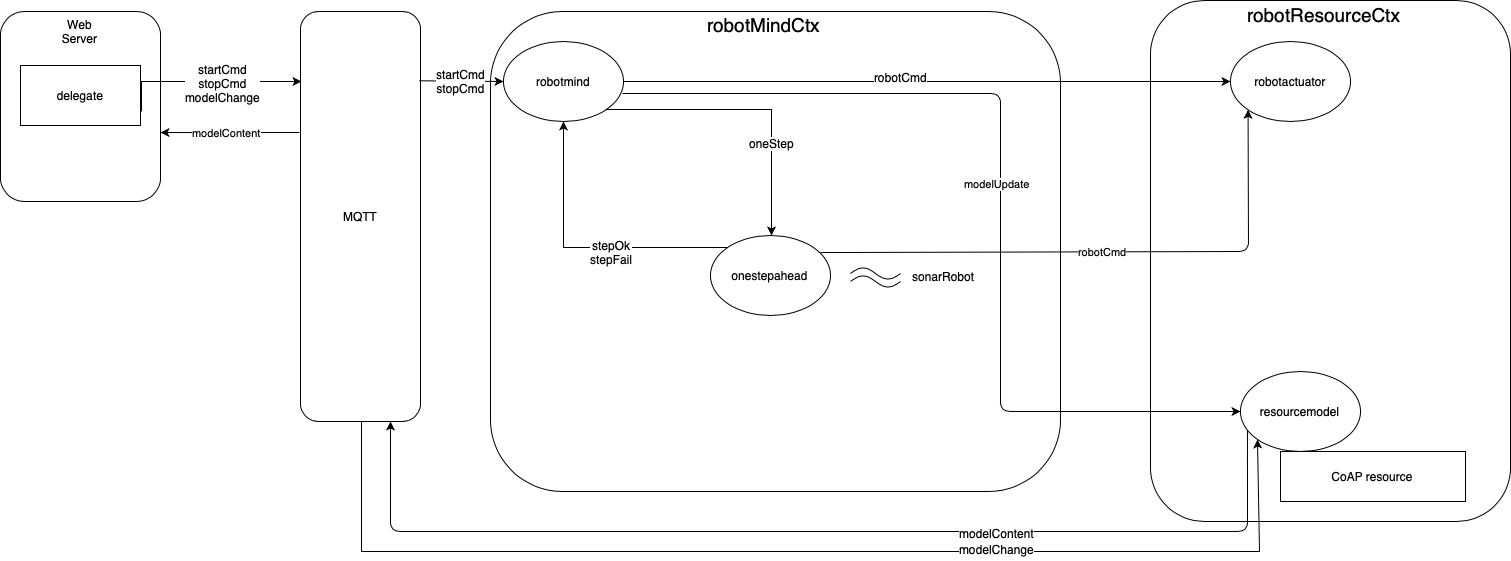
\includegraphics[width=\textwidth]{img/sprint3/arch_logica_3.png}
  \caption{L'architettura del sistema.}
  \label{fig:arch_logica_3}
\end{figure}

\subsection{Test plan}

Verificare il corretto funzionamento del sistema:

\begin{itemize}
\item alla pressione del tasto start/stop sulla web page il sistema parte/si ferma e lo stato della risorsa CoAP cambia coerentemente;
\item le informazioni visualizzate sulla web page corrispondano allo stato reale del sistema;
\end{itemize}{}

